\documentclass[a4paper]{scrartcl}
\usepackage[cm]{fullpage}
\usepackage{amsmath, amssymb, esint}
\usepackage{siunitx}

\usepackage{tikz, pgfplots}
\pgfplotsset{
    compat = 1.12,
    plot/.style = {
        axis lines = middle,
        clip = false
    },
    plot-scatter/.style = {
        only marks
    }
}

\begin{document}

\title{PHYS2114: Magnetic Hysteresis}
\author{ \\ \\ }
\date{2016-08-02}
\maketitle

\section{Introduction}
Please refer to the student notes of the experiment.

\section{Materials and Methods}
Please refer to the student notes, operating instructions and prework of the experiment.

Primary coil loops was specified to be \(n_p = 584\) and secondary to be \(n_s = 773\). The RC integrator's capacitor's capacitance was specified to be \(C = \SI{9.39}{\micro\farad}\), contrary to what is specified in the student notes. Mains AC frequency was measured to be \SI{50.0 \pm 0.1}{\hertz}.

Time series data was obtained both with and without the RC integrator at a \SI{100}{\kilo\hertz} sample rate, and then passed through a cubic Savitzky-Golay filter of window length 101 prior to being processed. This was to reduce noise and interpolate between the limited precision points from the oscilloscope. This data was then appropriately integrated using Simpson's rule following the method outlined below to obtain energy dissipated per cycle \(E\):

For the case with the RC filter, we follow off the prework with:
\begin{align*}
    E &= \frac{n_p}{n_s}\frac{R C}{R_p} \oint V_X \:\mathrm{d}V_{Y1} \\
    &\approx (\SI{78.04}{\milli\joule\per\volt\squared}) \int_{\SI{-0.01}{\second}}^{\SI{0.01}{\second}} V_X \frac{\mathrm{d}V_{Y1}}{\mathrm{d}t} \:\mathrm{d}t
\end{align*}

And without the RC filter, we have:
\begin{align*}
    E &= \frac{n_p}{n_s}\frac{1}{R_p} \oint V_X V_{Y2} \:\mathrm{d}t \\
    &\approx (\SI{377.7}{\milli\joule\per\volt\squared\per\second}) \int_{\SI{-0.01}{\second}}^{\SI{0.01}{\second}} V_X V_{Y2} \:\mathrm{d}t
\end{align*}

The volume of the iron core was also given to be \(V = 2 \pi r W h \approx \SI{18.9}{\centi\metre\cubed}\), though it is noted that it appeared to be a fair bit larger and rounder, possibly due to the primary and secondary coils.

\(V_Y\) values were converted to Teslas by either:
\begin{align*}
    B &= \frac{R C}{n_s W h} V_{Y1} \\
    &\approx (\SI{4.454}{\tesla\per\volt}) V_{Y1}
\end{align*}
or
\begin{align*}
    B &= \frac{1}{n_s W h} \int_0^t V_{Y2} \:\mathrm{d}t \\
    &\approx (\SI{21.56}{\tesla\per\volt\per\second}) \int_0^t V_{Y2} \:\mathrm{d}t
\end{align*}

Note that in both these cases, the values passed through integration without a boundary condition so there might have been an unknown constant offset. Because of this, we could only find the ``offset from the mean'' magnetic remanence \(B_r\) by measuring half the distance between the two opposite \(H = 0\) intercepts.

The above was repeated three times per voltage setting to obtain an estimate for error.

\section{Results}
\begin{figure}
    \centering
    \begin{tikzpicture}
        \begin{axis}[
            plot,
            xlabel = \({V_X}_{rms}\) (\si{\volt}),
            ylabel = \(E\) (\si{\joule})
        ]
            \addplot +[plot-scatter] table [x = Vrms, y = EPerCycle, col sep = tab] {data/with-integrator.tsv};
            \addplot +[plot-scatter] table [x = Vrms, y = EPerCycle, col sep = tab] {data/without-integrator.tsv};
        \end{axis}
    \end{tikzpicture}
    \caption{Energy dissipated per cycle (Blue: With integrator; Red: Without)}
    \label{fig:energy-per-cycle}
\end{figure}

\begin{figure}
    \centering
    \begin{tikzpicture}
        \begin{axis}[
            plot,
            xlabel = \(H_{max}\) (\si{\ampere\per\metre}),
            ylabel = \(B_r\) (\si{\tesla})
        ]
            \addplot +[plot-scatter] table [x = Hmax, y = Br, col sep = tab] {data/with-integrator.tsv};
            \addplot +[plot-scatter] table [x = Hmax, y = Br, col sep = tab] {data/without-integrator.tsv};
        \end{axis}
    \end{tikzpicture}
    \caption{Magnetic remanence (Blue: With integrator; Red: Without)}
    \label{fig:magnetic-remanence}
\end{figure}

\begin{figure}
    \centering
    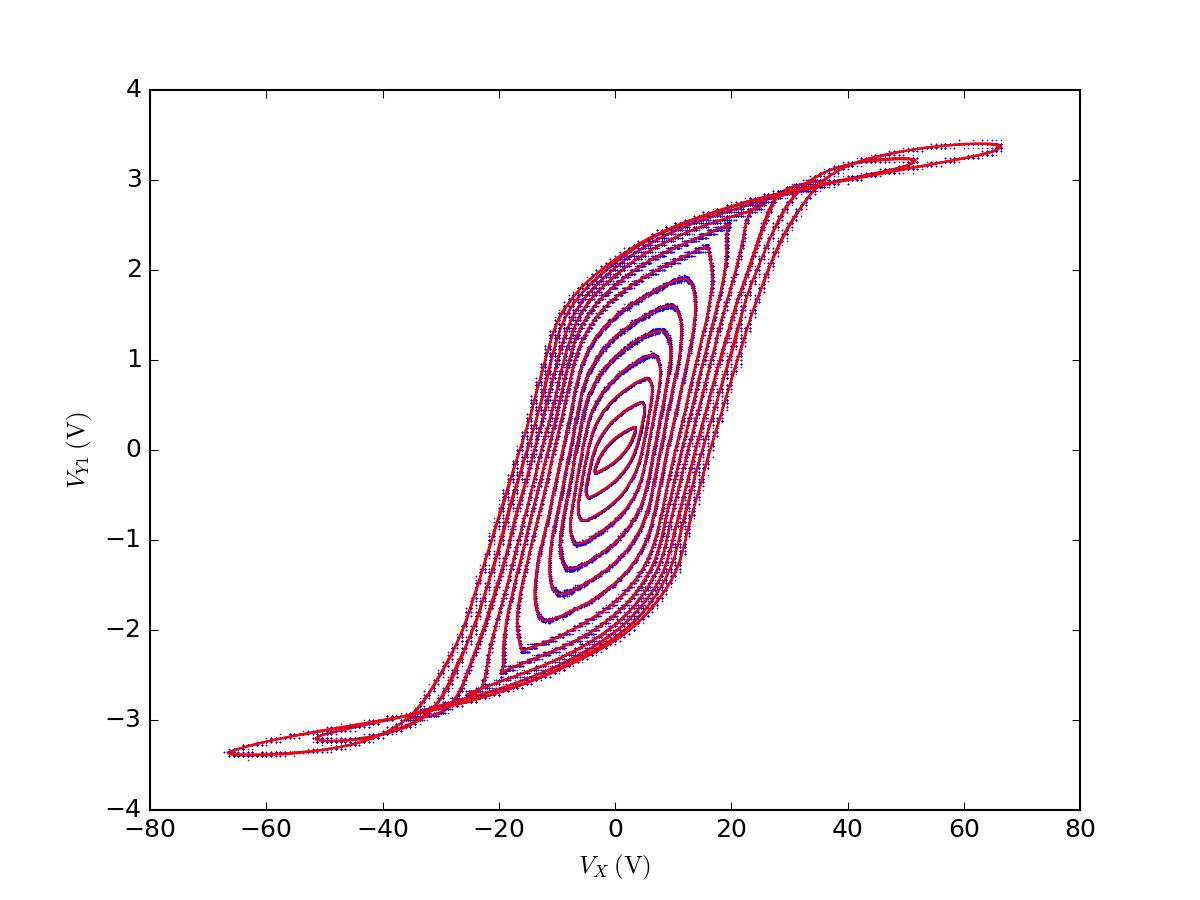
\includegraphics[height = 10cm]{with-integrator.png}
    \caption{Hysteresis loop shapes with the integrator (Blue: Samples; Red: Filtered curve)}
    \label{fig:with-integrator}
\end{figure}

\begin{figure}
    \centering
    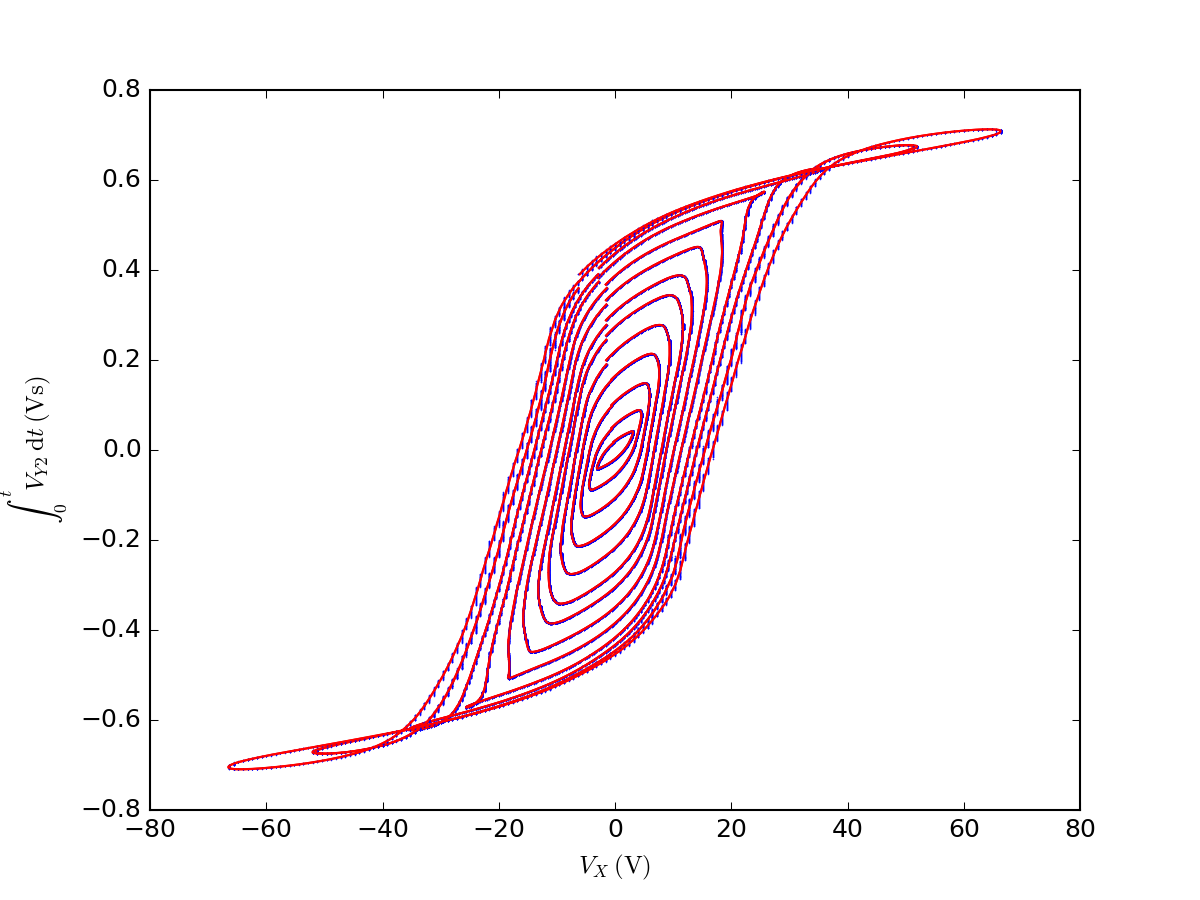
\includegraphics[height = 10cm]{without-integrator.png}
    \caption{Hysteresis loop shapes without the integrator (Blue: Samples; Red: Filtered curve)}
    \label{fig:without-integrator}
\end{figure}

\begin{figure}
    \centering
    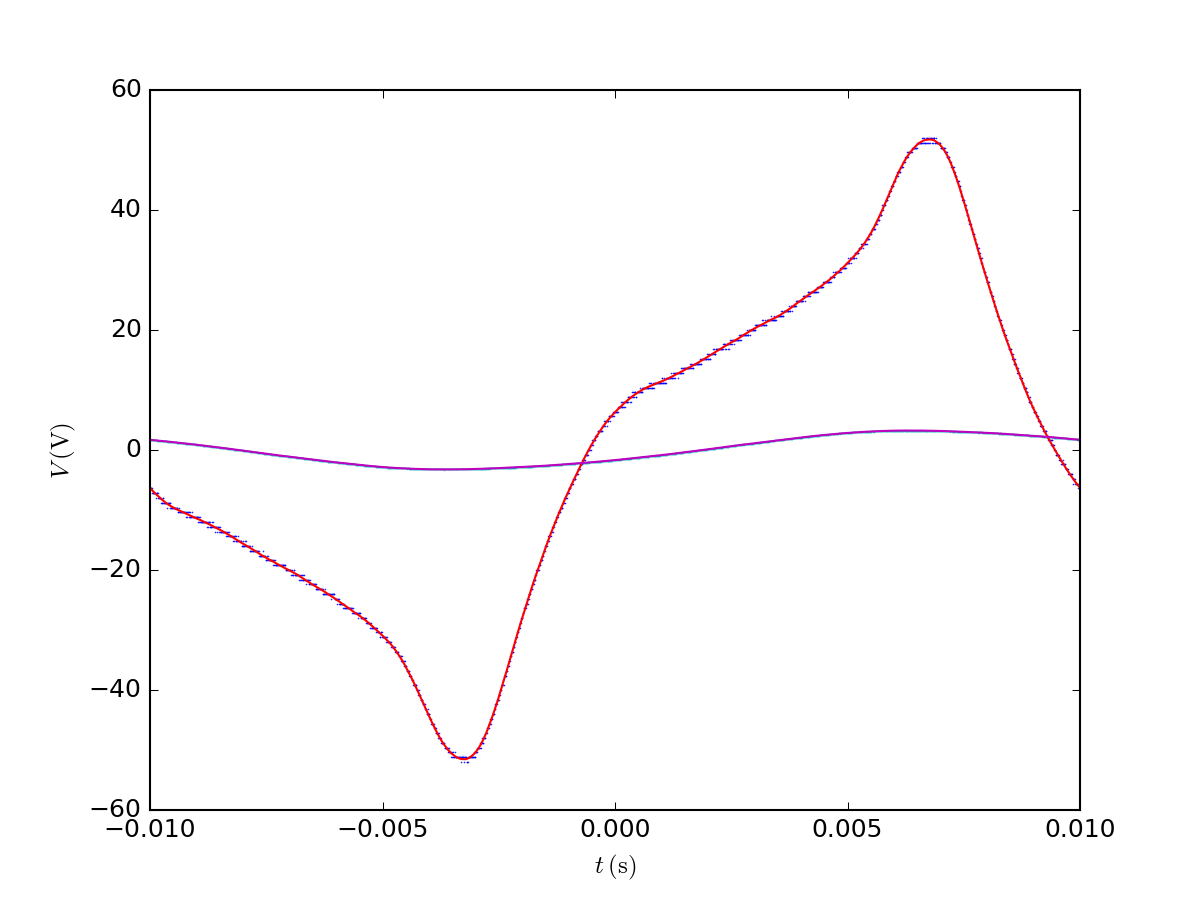
\includegraphics[height = 10cm]{with-integrator-waveform.png}
    \caption{Time series data of \({V_X}_{rms} = \SI{28}{\volt}\) with the integrator (Red/Blue: \(V_X\); Magenta/Cyan: \(V_{Y1}\))}
    \label{fig:with-integrator-waveform}
\end{figure}

\begin{figure}
    \centering
    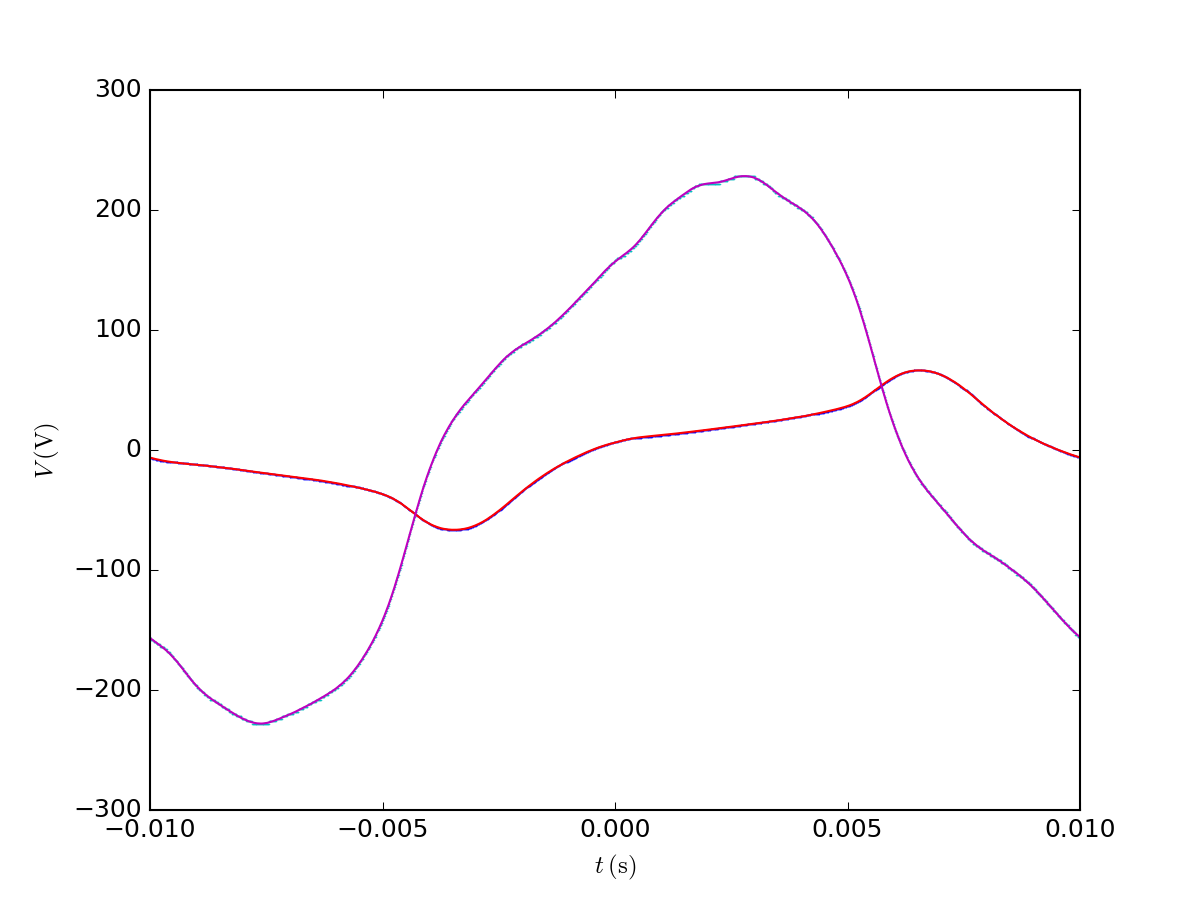
\includegraphics[height = 10cm]{without-integrator-waveform.png}
        \caption{Time series data of \({V_X}_{rms} = \SI{35}{\volt}\) without the integrator (Red/Blue: \(V_X\); Magenta/Cyan: \(V_{Y2}\))}
    \label{fig:without-integrator-waveform}
\end{figure}

The energy dissipated per cycle (Figure \ref{fig:energy-per-cycle}) increases sub-quadratically against input current initially before slowing down, with a ``knee'' at around \(\frac{\SI{17}{\volt}}{R_p} = \SI{8.5}{\ampere}\) RMS.

Magnetic remanence (Figure \ref{fig:magnetic-remanence}) initially increases linearly against peak magnetisation, ``knees'' at around \SI{8.2 \pm 0.1}{\tesla} at \SI{18}{\kilo\ampere\per\metre}, and then slows down to an almost flat gradient afterwards, with the highest recorded value being \SI{9.6 \pm 0.2}{\tesla} at \SI{62}{\kilo\ampere\per\metre}.

Both previous figures have uncertainties of around the same size as the plotted points. Points calculated from data measured without the integrator also resulted in less than \SI{10}{\percent}) larger energies and remanence.

Figures \ref{fig:with-integrator} and \ref{fig:without-integrator} show the hysteresis loops, with and without the integrator, respectively. The small discontinuities in Figure \ref{fig:without-integrator} are due to cumulative integration errors.

Figures \ref{fig:with-integrator-waveform} and \ref{fig:without-integrator-waveform} show the collected and filtered time series data, with and without the integrator, respectively. With the high input currents (\(\frac{\SI{28}{\volt}}{R_p} = \SI{14}{\ampere}\) and \(\frac{\SI{35}{\volt}}{R_p} \approx \SI{18}{\ampere}\)) respectively, it clearly shows non-sinusoidal shapes.

\section{Discussion}
The shapes of all the data are completely expected. The small discrepancy in the energy dissipated per cycle (Figure \ref{fig:energy-per-cycle}) and magnetic remanence (Figure \ref{fig:magnetic-remanence}) data between the measurements with and without the integrator most likely results from cumulative integration error, as also seen in Figure \ref{fig:without-integrator}.

However, most of the data appear to be in the wrong order of magnitude.

For example, take the maximum point collected on energy dissipated per cycle (Figure \ref{fig:energy-per-cycle}), the iron core dissipates \SI{12.3 \pm 0.5}{\joule} per cycle, and with the input at \SI{50.0 \pm 0.1}{\hertz}, this means a power of \SI{620 \pm 30}{\watt}, which is much too high for a transformer of this size.

Furthermore, the magnetic remanence (Figure \ref{fig:magnetic-remanence}) is also much too high - values typical of superconducting electromagnets, let alone permanent magnets.

Assuming all formulae used and measurements are correct, analysing the formulae points to two possible sources of error: \(R_p\) and \(n_s\).

Firstly, the reported RMS voltages across \(R_p\) ranged from \SI{2}{\volt} to \SI{35}{\volt}, corresponding to currents of \SI{1}{\ampere} to \SI{18}{\ampere}, almost double of what the wires between components are rated for (\SI{10}{\ampere}). A larger actual value of \(R_p\) would resolve this, and would affect other equations such as reducing the value of energy dissipated per cycle \(E\).

Next is \(n_s\). Assuming the primary coil impedance to be only a few Ohms at most (which is sound, since it appeared to be made out of metallic material), the voltage across it should be similar or less than \(V_X\). Using Figure \ref{fig:without-integrator-waveform} as an example with RMS \(V_X = \SI{35}{\volt}\) and the coil winding ratio \(\frac{n_s}{n_p} \approx 1.32\), the secondary coil voltage should be around \SI{46}{\volt} or less. Yet the measured RMS voltage was about \SI{160}{\volt}, which would mean the given \(n_s\) was too low or \(n_p\) to high. I chose a too low \(n_s\) here since a higher value would both decrease the absurdly high B-field values (along with the remanence), as well as decreasing \(E\), while a lower \(n_p\) would only do the latter.

\end{document}